\documentclass[main.tex]{subfile}

\begin{document}

\section{Methods} 
\label{sec:methods}

The following steps are performed with each step of the lab.

\begin{enumerate}
	\item 
		Set up the simulink module as follows. See the lab manual for details on
		setting up the block diagram. In short the HLRead/HLWrite blocks are the
		signal input/output of the DC motor system respectively. The ``count to
		degree'' block converts the input from the optical sensor (a optical
		encoder) to degrees to make the analysis easier to perform. The HLInitialize
		block sets up the DC motor system with initial properties.

		\begin{center}
			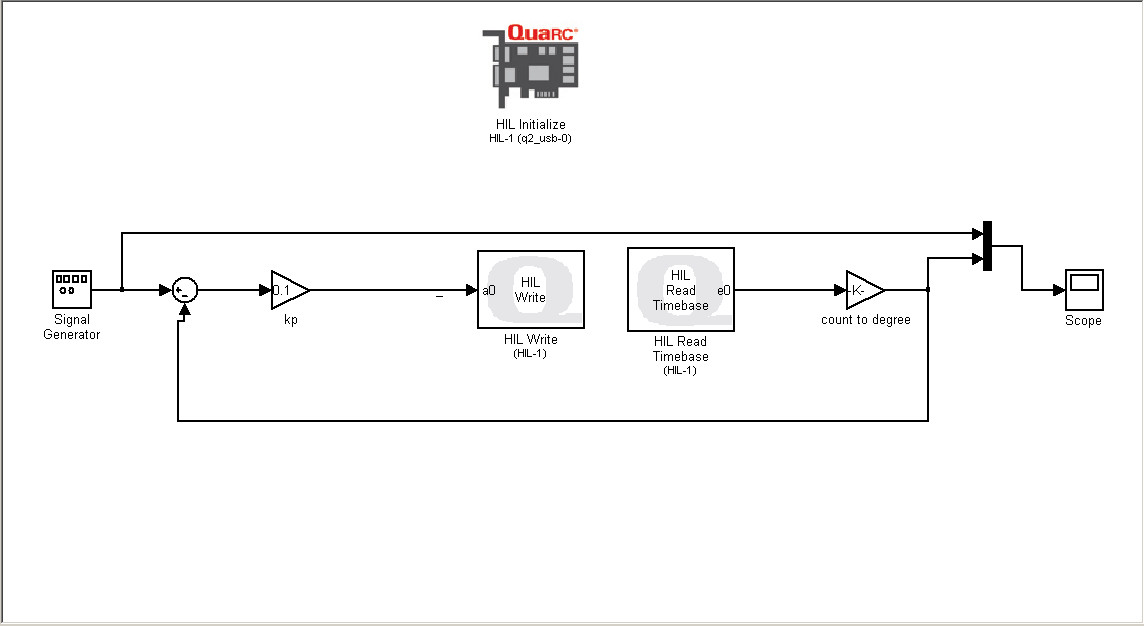
\includegraphics[width=4in]{step1}
		\end{center}

	\item
		Reset the arm (that is attached to the DC motor) to the $0^{\degree}$
		position.

	\item
		Modify the PID control constants ($K_p$,$K_i$,$K_d$) - add an integrator, or
		derivative term if necessary - according to the tables listed in
		\secref{results}.

	\item
		Run the simulink simulation and observe the system output using the scope
		tool. Stop the simulation after about three cycles.

	\item
		An image of the plots are saved for later analysis.

\end{enumerate}

% section methods (end)

\end{document}
